\documentclass[tikz, border=10pt]{standalone}
\usepackage{tikz}
\usetikzlibrary{angles, quotes}

\begin{document}

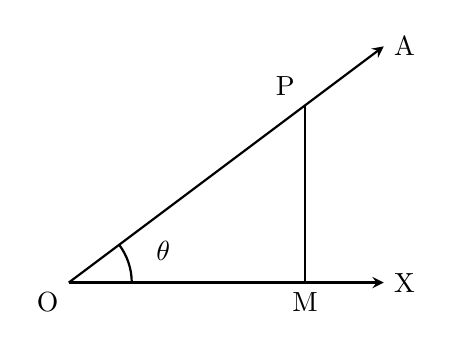
\begin{tikzpicture}[scale=1, >=stealth, line width=0.8pt]

% Define coordinates
\coordinate (O) at (0,0);
\coordinate (X_end) at (4,0);
\coordinate (A_end) at (4,3);
\coordinate (M) at (3,0);
\coordinate (P) at (3,2.25); % Point on OA such that PM is vertical

% Draw rays OA and OX
\draw[->] (O) -- (A_end) node[right] {A};
\draw[->] (O) -- (X_end) node[right] {X};

% Draw perpendicular segment PM
\draw (P) -- (M);

% Draw angle arc for theta
\draw (0.8,0) arc (0:36.87:0.8);

% Place labels
\node[below left] at (O) {O};
\node[above left] at (P) {P};
\node[below] at (M) {M};
\node at (1.2, 0.4) {$\theta$};

\end{tikzpicture}

\end{document}
